\documentclass[12pt,a4paper]{article}

\usepackage[sfdefault,lf]{carlito}
\usepackage[hidelinks]{hyperref}  % instead of \usepackage[spaces,obeyspaces,hyphens]{url}
\usepackage[natbibapa]{apacite}

\usepackage[english]{babel} % if your work is in English
%\usepackage[finnish]{babel} % jos työsi on suomeksi
\usepackage[utf8]{inputenc}
\usepackage{times}
\usepackage{setspace}
\linespread{1.5}
\usepackage[top = 2.8cm, bottom = 3.5cm, inner = 3cm, outer = 3cm, headheight = 15pt]{geometry}
\usepackage{lastpage}
\usepackage{amssymb}
\usepackage{amsthm}
\usepackage[mathscr]{eucal}
\usepackage{mathrsfs}
\usepackage{enumitem}
\usepackage{bm}
\usepackage{multirow}
\usepackage{array}
\usepackage{ragged2e}
\usepackage{etoolbox}
\usepackage{environ}
\usepackage[hang,flushmargin]{footmisc}
\usepackage{graphicx}

\usepackage{pdfpages}%%%% include pdf files
\usepackage{amsmath}
\usepackage{colortbl}
\usepackage[font=small,labelfont=bf, labelsep=period, format=hang, singlelinecheck=false, justification=raggedright, textformat=period]{caption}
\usepackage{titlesec}
\usepackage[nottoc]{tocbibind}
\usepackage[titletoc]{appendix}
\usepackage{tikz}

\graphicspath{ {./figures/} }

\captionsetup[table]{position=above}
\captionsetup[figure]{position=below}

\bibliographystyle{apacite}


\usepackage[titles]{tocloft} % no bold or dots toc
\renewcommand{\cftsecfont}{\mdseries}
\renewcommand{\cftsecpagefont}{\mdseries}
\renewcommand{\cftdot}{}

\renewcommand{\doiprefix}{}
    \newcommand{\doi}[1]{https://doi.org/#1}

\titlespacing\section{0pt}{12pt plus 4pt minus 2pt}{0pt plus 2pt minus 2pt}
\titlespacing\subsection{0pt}{12pt plus 4pt minus 2pt}{0pt plus 2pt minus 2pt}
\titlespacing\subsubsection{0pt}{12pt plus 4pt minus 2pt}{0pt plus 2pt minus 2pt}
    
%%%%%%%%%%%%%%%%%%%%%%%%%%%%
%%% Your personal  info %%%%
%%%%%%% Omat tietosi %%%%%%%
%%%%%%%%%%%%%%%%%%%%%%%%%%%%
% Pääotsikko Title
\newcommand{\thetitle}{
Title of your work
}
%%%%%%%%%%%%%%%%%%%%%%%%%%%%
% Alaotsikko - Subtitle
\newcommand{\thesubtitle}{
Subtitle if needed
}
%%%%%%%%%%%%%%%%%%%%%%%%%%%%
% Nimesi - Your name FirstName Familyname
\newcommand{\theauthor}{
First-Name Surname
} % Etunimi Sukunimi
%%%%%%%%%%%%%%%%%%%%%%%%%%%%
%%%%%%%%%%%%%%%%%%%%%%%%%%%%

%%% headings and pagenumbers &&&&
\usepackage{fancyhdr}
\pagestyle{fancy}
\fancyhf{} % sets both header and footer to nothing
\fancyheadoffset{0cm}
\renewcommand{\headrulewidth}{0pt} 
\renewcommand{\footrulewidth}{0pt}

%%%%%%%%%%%%%%%%%%%%%%%%%%%%
%%%%%%% thesis begins %%%%%%
%%%%%% opinnäyte alkaa %%%%%
%%%%%%%%%%%%%%%%%%%%%%%%%%%%
\begin{document}
\setlength{\parindent}{0pt}
\setlength{\bibindent}{1.25cm}

\urlstyle{same}
\newcommand{\changefont}{%
    \fontsize{11}{12}\selectfont}

% kansilehti - coverpage
\pagestyle{empty}
\begin{center}

\includegraphics{figures/univaasa-logo-opt_cover.jpg}

\begingroup

{\Large
{\ Nahid Hasan Sarkar}\bigskip
}


\textbf{\LARGE{\ Developing a Forecasting-Based Decision-Support Framework for Third-Party Delivery Sales Optimization}}\bigskip

\bigskip

\end{center}

\endgroup
\vspace*{\fill}
\bigskip
 
\begin{flushright}

School of Technology and Innovation
\\
Industrial Engineering and Management
\\
Industrial Systems Analytics

\end{flushright}

\begin{flushright}\end{flushright}
\vspace*{\fill}

\begin{center}
Vaasa 2026
\end{center}

% sivunumerointi - page numbering
\newpage\pagestyle{fancy}
\pagestyle{fancyplain} % Makes all pages in the document conform to the custom headers and footers
\fancyhead[L]{}% Empty left header
\fancyhead[C]{\changefont \thepage} % Page numbering for center header with smaller font  
\fancyhead[R]{}% Empty right header
\fancyfoot[L]{}% Empty left footer
\fancyfoot[C]{}% Empty center footer
\fancyfoot[R]{}% Empty left footer


%%%%%%%%%%%%%%%%%%%%%%%%%%%%%
%%% abstracts start here %%%%
%%%%%%%%%%%%%%%%%%%%%%%%%%%%%

%%%% comment or remove next lines, if abstracts are not needed

%%{
    

\begin{table} %[]
\small
\begin{tabular}{llll}
\hline
\multicolumn{4}{l}{\textbf{VAASAN YLIOPISTO}}                                        \\
\multicolumn{4}{l}{\textbf{Xxx yksikkö}}                                             \\
\textbf{Tekijä:}           & \multicolumn{3}{l}{\theauthor}                    \\
\textbf{Tutkielman nimi:}  & \multicolumn{3}{p{10cm}}{\thetitle : \thesubtitle} \\

\textbf{Tutkinto:}         & \multicolumn{3}{l}{XXX}                                 \\
\textbf{Työn ohjaaja:}     & \multicolumn{3}{l}{Etunimi Sukunimi}                    \\

\textbf{Valmistumisvuosi:} & 20XX          & \textbf{Sivumäärä:}         & \pageref{LastPage}        \\ \hline
\multicolumn{4}{l}{\textbf{TIIVISTELMÄ:}}                                            \\
\multicolumn{4}{p{14.5cm}}{

Either one or both abstracts. One abstract must fit in one page. 
} \\
\hline
\multicolumn{4}{l}{\textbf{Avainsanat:} Finto: \url{http://finto.fi/yso/fi/?clang=fi\&anylang=on} }                                                    
\end{tabular}
\end{table}


}% tiivistelmä
%\null\newpage % new page after abstract
{
\begin{table}[!ht]
\fontsize{11pt}{11pt}\selectfont
\setstretch{1}

\begin{tabular}{llll}
\hline

\multicolumn{4}{l}{\textbf{VAASAN YLIOPISTO}} \\ \\
\multicolumn{4}{l}{School of Technology and Innovation} \\ \\

Author: &
\multicolumn{3}{l}{Nahid Hasan Sarkar} \\ \\

Thesis title: &
\multicolumn{3}{l}{\textbf{Developing a Forecasting-Based Decision-Support Framework for Third-Party Delivery Sales Optimization}} \\ \\

Degree: &
\multicolumn{3}{l}{Master of Science in Technology} \\ \\

Degree Specialization: &
\multicolumn{3}{l}{Industrial Systems Analytics} \\ \\

Supervisor: &
\multicolumn{3}{l}{Jyri Naarmala} \\ \\

Year of graduation: &
2026 &
Number of pages: &
\pageref{LastPage} \\                                                               \\

\hline
\\
\multicolumn{4}{l}{\textbf{ABSTRACT:}}                                               \\ \\

\multicolumn{4}{p{14.5cm}}{

This study develops a data-driven decision-support framework to optimize third-party delivery platform sales in the Quick Service Restaurant (QSR) industry. With the rapid growth of platforms such as Wolt and Foodora, large volumes of transactional data are generated, offering opportunities for advanced analytics. However, many businesses do not fully utilize this data for forecasting and decision-making.

The research follows a Design Science Research (DSR) approach to design and evaluate a framework that integrates data preprocessing, demand forecasting, and profit optimization. Historical sales data from Wolt and Foodora are first cleaned and integrated into a unified dataset. A Prophet time series model is then applied to forecast platform-level demand, capturing trend and weekly seasonal patterns. The forecasting results are further used as input for an optimization model that generates profit-oriented decision recommendations under practical constraints such as delivery capacity and platform fees.

The proposed framework is evaluated through simulation and back-testing using historical data. Forecasting performance is assessed using standard accuracy metrics including MAE, RMSE, and MAPE. The results show that the proposed approach can improve decision-making by providing more accurate demand predictions and more efficient platform allocation strategies. The integration of predictive and prescriptive analytics demonstrates clear potential for improving profitability and operational efficiency.

Overall, the study contributes to the field of business analytics by combining predictive and prescriptive analytics into a unified decision-support framework for multi-platform food delivery operations.

} \\

\hline

\multicolumn{4}{p{14.5cm}}{
\textbf{Keywords:} Demand forecasting, Prophet model, decision support systems, optimization, food delivery platforms
} 


\end{tabular}
\end{table}
}% abstract

 %new page after abstract \null\newpage

 
%%%%%%%%%%%%%%%%%%%%%%%%%%%%%
%%%%% abstracts end here %%%%
%%%%%%%%%%%%%%%%%%%%%%%%%%%%%


\section*{Declarations}

\subsection*{AI usage}

During the preparation of this thesis, I have used AI-based tools.

\begin{enumerate}
    \item \textbf{AI tool name: ChatGPT (OpenAI)}
    
    \begin{enumerate}
        \item Purpose of use: Sentence restructuring and proofreading.
        
        \item Explanation of the use of the tool: ChatGPT was used for language refinement and improving clarity in writing.
    \end{enumerate}
    
    \item \textbf{AI tool name: Grammarly}
    
    \begin{enumerate}
        \item Purpose of use: Checking grammar, spelling, and punctuation.
        
        \item Explanation of the use of the tool: Grammarly was used to correct grammar, spelling mistakes, and missing punctuation.
    \end{enumerate}
\end{enumerate}


% sisällysluettelo - table of contents
\newpage
\tableofcontents

% kuviot - figures ... add \newpage and remove comment, if needed
%{\let\oldnumberline\numberline \renewcommand{\numberline}{\figurename~\oldnumberline} \listoffigures}

% taulukot - tables
% add \newpage and remove comment, if needed
%{\let\oldnumberline\numberline \renewcommand{\numberline}{\tablename~\oldnumberline}     \listoftables }

% text settings
\setlength{\parskip}{1.8em}

%%%%%%%%%%%%%%%%%%%%%%%%%%%%%%%%%%
% ensimmäinen luku - first chapter
\newpage
\section{Introduction}

\subsection{Background of the Study}

Due to digitalization and the change of behavior of consumer in QSR industry for the last few years \citep{govender2024digital} have been transformed a lot. Perhaps the biggest change has been from third-party delivery platforms, which have transformed customer relationships with restaurants \citep{meemken2022research}. Mobile applications such as Wolt and Foodora have become core players in the food service ecosystem and, through them, customers can place orders for meals over this application quickly and receive on-demand delivery within minutes \citep{simonovits2022uberisation, tuomi2023riding}.

Urbanization, rising smartphone usage and a preference for convenience have contributed to the proliferation of these platforms. This demand has increased consumer expectations of speed, reliability and digitally accessible food delivery services -- particularly in urban markets \citep{siddiqi2024investigating}. Consequently, QSR businesses found themselves heavily reliant on third-party platforms to serve as a primary or secondary sales channel. The new landscape has not only broadened market access but also added complexity to restaurants both operationally and strategically \citep{sun2022too}.

One of the key ramifications of this platform-based model is the massive data it creates. Transactions processed on a platform, such as Wolt and Foodora, generate extensive data logs with information about the time of orders, order values, product selection, time at which goods were delivered and service provider fees per platform \citep{nayak2024future}. In this process, you end up with historical datasets that form insights on customer behavior patterns, seasonal demand variations and comparative performance of the platform. That data, theoretically, is a valuable basis for predictive analytics and decision making.

Nonetheless, this data is readily available but many QSRs do not leverage it to its full potential \citep{almeida2023time,nayak2022restaurant} Data is in fact, usually used for the purpose of describing events that already happened (like looking back at previous sales or coming up with simple reports). Although these descriptive insights are informative in that they provide information about what happened, they do not predict future outcomes or how to intervene to get better outcomes \citep{ma2020making, roy2022complete}. Between making data available and providing intelligence to act upon there exists an insurmountable gulf.




This rising standard is reflected through the same increasing competitive nature of the QSR industry \citep{altenburger2019artificial}. Between these managers are various delivery platforms that restaurants need to work with at once, each having different commissions, customer bases and promotional dynamics \citep{feldman2023managing}. For example, deciding how to spread budgets by channel, timing of sales/discounting or responding to demand volatility has a direct effect on revenue and bottom line. It is sub-optimal to simply be decisioning these based on gut feels or historical averages \citep{cai2023marketing}.

Data-driven decision making has emerged as an important capability in this context. Businesses are progressively also expected to shift from descriptive analytics towards predictive and prescriptive \citep{berkhout2024revisiting}. On the one hand, predictive analytics allows organizations to make predictions about future demand based on historical data; while prescriptive analytics takes it further and recommends which actions should be taken to achieve objectives (e.g., maximize profit or improve service efficiency) rather than reporting only future benefits [4].

For QSRs existing on third-party platforms, the combination with these analytic methods has great potential \citep{li2024criticality}. Through the systematic analysis of platform data, businesses can spot demand patterns with respect to time and platforms, predict future sales trends well in advance, as well as take note to undertake preemptive actions \citep{wu2025does}. For example, PR frameworks can help in generating accurate demand forecasts leading to better staffing, inventory planning and promotional strategies whilst optimization models can be used for platform level decision making improvements \citep{shen2025jd}.


However, there is still a shortage of frameworks that combine the challenges of data integration, forecasting and decision optimization in one coherent framework \citep{khan2025model}. The tools or expertise required to derive actionable insights from raw data that is useful for managerial decisions are hard to come by for many businesses \citep{zhang2025timeraf}. Hence, this study is driven by the purpose of establishing a data-driven framework that combines both availability and usability of data in decision-making within the context of QSRs, which is an essential practice for gainful business implementation as well as an addition to the existing field of business analytics.

\subsection{Problem Statement}

With a more competitive third-party delivery marketplace, and the transaction data of sales widely available with merchants \citep{ogunmokun2025role}, coming up with a tactical plan from the ground-level (sales data) can be much harder for many businesses \citep{taylor2017new}. For HungryHub Oy, big amounts of transactional data is continuously produced via platforms like Wolt and Foodora \citep{mbare2023psychosocial}. So we gather data on order trends, customer preferences, how the platform is performing.


But the current utility of this data is still frozen in time. In the practice it is mainly identifiable as descriptive analysis like using historical trends of sales for reporting purposes to create simple reports \citep{wolniak2023concept}. Though this gives a glimpse into how things were, it does not help plan for the future. Consequently, important operational and strategic choices—e.g., allocation of sales on platform-level, promotion planning and demand forecasting—are not sufficiently backed by systematic analytic approaches \citep{groene2024introduction}.


These limited use of advanced data creates a massive divide between the data available and decision making effectiveness. So, HungryHub is unable to provide a good demand forecasting for future across multiple platforms without predictive models. Moreover, the company is missing prescriptive tools which provide possible overall optimal decisions to maximize profit from forecast. Rationality might be replaced with intuition or naive assumptions in decision-making, which can result in substantive inefficiencies and missed opportunities culminating in unsatisfactory financial outcomes.


This constraint lessens the companys ability to preemptively react to fluctuations in demand and optimize their operational functionality across delivery channels in a highly competitive QSR space \citep{racine2022college}. Hence, the main issue tackled in this work is the lack of a unified analytical framework incorporating data preparation, demand forecasting, and decision optimization.

\subsection{Research Objectives}

The main aim of this research is creation of a prescriptive decision support system to optimize the sales of third party delivery platform. In particular, the study will seek to combine sales data on websites like Wolt and Foodora into a single analytical dataset that will allow performing a thorough analysis. 

Based on this, the research aims at constructing and testing the models of forecasting that will have the capacity to predict the demand at the platform level. Moreover, the study aims at converting these demand predictions into profit-driven decision makers by developing an optimization model. Lastly, the study will evaluate the possible business consequences of the proposed framework through simulation or back-testing, to determine the effectiveness of the proposed framework in enhancing decision-making and the overall sales performance.

\subsection{Research Questions}

The study addresses the following research questions:

\begin{itemize}
    \item \textbf{RQ1:} How can sales data from third-party delivery platforms be structured into a unified analytical dataset for decision-making?
    
    \item \textbf{RQ2:} Which forecasting approach provides the most accurate predictions of platform-level demand?
    
    \item \textbf{RQ3:} How can demand forecasts be transformed into profit-oriented decision recommendations?
    
    \item \textbf{RQ4:} What is the potential business impact of a prescriptive decision-support framework in optimizing platform sales performance?
\end{itemize}

\subsection{Scope and Limitations}

This research project aims at developing a data-driven decision support model of third party delivery sales at HungryHub Oy. Only sales data of two platforms, Wolt and Foodora, is analyzed. The research primarily investigates platform-level performance such as sales trend and demand prediction.

The study involves the cleaning and integration of the data, the formulation of forecasting models and the formulation of a simple profit-based decision model. The outcomes are measured on the basis of simulation or back-testing of the possible impact on business.

But there exist certain limitations. Other channels of sales (dine-in or takeaway) are not part of the study. It also does not discuss such operational aspects as kitchen management, staffing or delivery logistics. Moreover, the framework is not used as an active system, but merely tested with historical data. These constraints allow maintaining the research narrow and within the scope of a Master’s thesis.

\subsection{Structure of the Thesis}
The structure of this thesis is summarized in Table~\ref{tab:thesis_structure}.

\begin{table}[ht]
\centering
\renewcommand{\arraystretch}{1.5}
\begin{tabular}{|c|p{10cm}|}
\hline
\textbf{Chapter} & \textbf{Description} \\ \hline

\textbf{Chapter 1} &
Introduction to the study, including background, problem statement,
research objectives, research questions, and scope. \\ \hline

\textbf{Chapter 2} &
Theoretical background covering business analytics, demand forecasting,
decision-support systems, and Design Science Research. \\ \hline

\textbf{Chapter 3} &
Research methodology, including research approach, data collection,
and analysis methods. \\ \hline

\textbf{Chapter 4} &
Data preparation and development of forecasting models. \\ \hline

\textbf{Chapter 5} &
Design of the decision-support framework and evaluation using simulation
or back-testing. \\ \hline

\textbf{Chapter 6} &
Discussion of results, key findings, and practical recommendations. \\ \hline

\textbf{Chapter 7} &
Conclusion, including summary, limitations, and suggestions for future research. \\ \hline

\end{tabular}
\caption{Structure of the Thesis}
\label{tab:thesis_structure}
\end{table}% Introduction, Johdanto eg jne

%%%%%%%%%%%%%%%%%%%%%%%%%%%%%%%%%%
% toinen luku - second chapter
\newpage
\section{Literature Review}

In recent years, the restaurant industry has changed significantly due to digital technology and data availability \cite{almeida2023time}. Restaurants now operate through multiple sales channels such as dine-in, mobile applications, and third-party delivery platforms \cite{li2024criticality}. These channels generate large amounts of data that can help businesses better understand customer behavior and improve performance \cite{marciano2020big}. Studies show that integrating data from different sources supports better decision-making in areas such as pricing, promotions, and demand planning \cite{wu2025does}.

The concept of Business Analytics has been widely discussed in the literature as a key enabler of data-driven decision-making. It involves the use of data, statistical methods, and analytical techniques to support organizational decisions \cite{liu2023review}. By transforming raw data into meaningful insights, business analytics helps organizations analyze past performance, predict future trends, and make informed decisions \cite{soldic2025business}. Existing studies commonly classify business analytics into three categories: descriptive, predictive, and prescriptive analytics \cite{sharma2022analytics}. Descriptive analytics focuses on analyzing historical data, while predictive analytics is used to forecast future outcomes \cite{almeida2023time}. In contrast, prescriptive analytics provides recommendations for optimal actions by combining data analysis with optimization models \cite{frazzetto2019prescriptive}. Research highlights that prescriptive analytics plays a critical role in improving decision-making by enabling organizations to choose the best possible actions based on data-driven insights \cite{berkhout2024revisiting}. 

Apart from forecasting and optimization, recent studies highlight the need for integrated decision support systems in enhancing the operational efficiency and strategic planning \citep{roy2022restaurant}. Decision support frameworks use a combination of data management, analytical models, and visualization to help organisations make informed choices and decisions based on evidence and in a timely fashion \citep{tajeddini2026smart}. For restaurants, these systems can be beneficial in their ability to track sales data, understand customer trends, and assess profitability on each platform \citep{shah2025exploring}. Additionally, as digital platforms for food delivery become popular, researchers point out the need to develop analytical frameworks that can effectively process vast amounts of transactional data in real-time on a scalable platform \citep{majid2019role}. Therefore the use of predictive analytics in the food service sector in conjunction with business intelligence and decision support systems is an area of research that has emerged as a significant challenge for achieving competitiveness.

Despite these advancements, there are still research gaps in the literature \cite{zhang2025timeraf}. Many studies focus only on predictive or prescriptive analytics separately rather than integrating them \cite{frazzetto2019prescriptive}. There is also limited research specifically focused on the restaurant industry, especially small and medium-sized enterprises \cite{li2024criticality}. In addition, multi-channel sales are often studied independently instead of as interconnected systems \cite{furst2022multi}. However, despite these contributions, most existing research focuses on either data analysis, prediction, or optimization separately. There is limited research that integrates all these components into a unified framework, especially in the context of multi-channel sales in the restaurant industry. Furthermore, many studies do not address the practical challenges faced by small and medium-sized businesses.

Therefore, this study aims to address these gaps by developing a prescriptive decision intelligence framework that combines data integration, predictive analytics, and optimization techniques. The case of HungryHub Oy provides a practical context to demonstrate how such a framework can support better decision-making and improve multi-channel sales performance.


\subsection{Demand Forecasting in Food Delivery Platforms}

Demand forecasting is very important for restaurants, especially those using online delivery platforms \citep{chae2024value}. It helps businesses estimate how many orders they will receive in the future \citep{li2025demand}. This allows them to plan better, reduce waste, and improve service.

\textbf{Restaurant Demand Forecasting}

Previous research has investigated predicting restaurant demand based on past sales data \citep{shinoda2021prediction, fernandes2021data}. Methods such as daily or weekly trends observed via algebraic solutions such as simple and time-series models \citep{wang2024deep}. These methods ultimately help avoid high- and low-demand periods. Some additional techniques include machine learning models for improving prediction \citep{rasheed2023improving}. These models may also take into account additional factors, such as holidays, promotions, or special events. Demand Forecasting Demand forecasting — in a nutshell — assists restaurants to plan inventory and operations better.

\textbf{Online Delivery Analytics}

With the growth of platforms like Wolt and Foodora, researchers have started to focus on online delivery data \citep{mbare2023psychosocial}. These platforms generate detailed data about customer orders, timing, and preferences. Studies show that this data can be used to understand customer behavior and platform performance \citep{geissinger2022sharing}. For example, businesses can see which platform performs better at certain times or which products are more popular. However, most studies focus either on forecasting or on data analysis separately. There is still a lack of research that combines forecasting with decision-making. This study aims to connect these two areas by using forecasts to support better business decisions.


\subsection{Time Series Forecasting Methods}

Time series forecasting methods are widely used to predict future values based on historical data \citep{kolambe2024forecasting}. In the context of this study, these methods are applied to forecast platform-level sales using past transaction data. Different approaches can be used depending on the data characteristics and complexity.

\textbf{ARIMA Models}

ARIMA:AutoRegressive Integrated Moving Average method is widely used classical statistical method for time series forecasting \citep{arumugam2023time}. It does this by identifying patterns in historical data trends, seasonality, to make predictions of future values \citep{bektemyssova2022time}. ARIMA works great on time series data that displays consistent patterns over a period of time. This makes them pretty easy to implement and widely understood. Yet, they can not generalize well in ultra-complex or non-linear datasets — that are present in real-world business context \citep{albeladi2023time}.

\textbf{Machine Learning Approaches}

In recent years, machine learning methods have gained considerable attention in forecasting tasks. This includes models ranging from linear regression, decision trees, random forests to neural networks \citep{masini2023machine}. Machine learning, as opposed to conventional models, can learn complex or non-linear relationships in the data \citep{ahamed2023machine}. They can, too, consist of several input variables, which is classified according to time, promotions or external factors. This makes them more versatile, as well as usually more precise than conventional techniques \citep{benti2023forecasting}. On the other hand, machine learning models tend to require a greater amount of data and fine-tuning. They also tend to be harder to interpret than simpler statistical models.

\textbf{Prophet Forecasting Model}

Prophet is a business time-series forecasting model developed by Facebook (Meta) \citep{sivaramakrishnan2022forecasting}. This is specifically useful when data has a high seasonality and missing values \citep{anand2024comparative}. Overview: ProphetThis model trends and seasonality easily and flexibly in addition to holidays. It is user-friendly and achieves decent performance on several realistic datasets, particularly those with daily or weekly periodicity \citep{najem2026hybrid}. This research uses Prophet as one of the key forecasting methods applied because it has easy handling of seasonality and also can easily be used in business contexts.


\subsection{Decision Support Systems}

Decision Support Systems (DSS) are computer-based tools that help managers and decision-makers make better and more informed decisions \citep{fernando2022decision}. These systems combine data, analytical models, and user-friendly interfaces to support problem-solving and planning in organizations \citep{triantafyllou2024decision}. 

In business contexts, DSS frameworks typically consist of three main components \citep{bernardi2024conversing}. The first is the data component, which includes internal and external data sources such as sales data, customer information, and market data. The second is the model component, which involves analytical methods such as forecasting models, optimization techniques, or simulation models. The third is the user interface, which allows decision-makers to interact with the system and interpret the results.

DSS frameworks are designed to support different types of decisions, including structured, semi-structured, and unstructured problems \citep{alojail2023informed}. In many cases, they are used to analyze different scenarios, evaluate possible outcomes, and recommend actions \citep{ghiani2024integrating}. This makes them especially useful in dynamic business environments where decisions must be made under uncertainty.

Forecasting and optimization are combined in the DSS as per this study. The system requires the past sales information, it forecasts demand and makes a decision recommendation on the basis of the forecasts. This assists businesses in leaving behind mere knowledge of past data to making proactive and data-driven decisions. In general, DSS are significant in enhancing efficiency, reducing uncertainty, and assisting superior strategic and operational decisions within the contemporary organizations.


\subsection{Profit Optimization in Digital Platforms}

Profit optimization is an important topic in digital platform-based businesses, especially in industries like food delivery where multiple platforms, pricing structures, and customer behaviors interact \citep{deng2022profit}. In such environments, businesses aim to maximize revenue or profit by making better decisions related to pricing, promotions, and sales allocation across platforms.

Pricing optimization is an important research area \citep{rangaswamy2020role}. According to \cite{ali2024investigating}, using pricing strategies, such as discounts and promotional offers, can greatly impact demand for the customers. Dynamic pricing and targeted promotion strategies are common in digital platforms to lure customers and increase order volume \citep{kopalle2023dynamic}. Nevertheless, continuously discounting their products may erode their profit margins thus companies should find a reasonable trade-off between higher demand and profitability \citep{nowak2024dynamic}.

Allocation optimization is another important area. For multiple delivery platforms, this means deciding how much of their focus, resources or promotion should be allocated to each platform \citep{ashraf2023optimal}. Different platforms may have different commission fees, customer reach and demand patterns. More specifically, literature shows that allocating resources optimally increases the overall output by focusing on the channels that are more profitable \citep{alnaggar2021crowdsourced}.

Optimization models, such as linear programming and simulation-based approaches, are commonly used to support these decisions \citep{abolghasemian2025simulation}. These models take inputs such as demand forecasts, pricing strategies, and cost structures to recommend actions that maximize profit or revenue under certain constraints. In many cases, profit optimization is closely linked with demand forecasting. Accurate forecasts provide the foundation for better optimization decisions \citep{verma2024transforming}.

In the absence of sound predictions, optimization models can deliver ineffective or impractical suggestions. Profit optimization is combined with forecasting in this study to develop prescriptive decision-support model. It is not only aimed at anticipating the future demand but also proposing actions that can enhance financial performance across digital platforms of delivery. This integrated strategy assists companies to make better, evidence-based decision-making in a competitive platform world.


\subsection{Research Gap}

Despite the increasing body of research on the topic of demand forecasting and digital platform analytics, a number of crucial gaps remain. Most of the studies are dedicated to the demand forecasting of restaurants with the help of the statistical or machine learning models, whereas others analyze the behavior of customers and their performance in online delivery services. Nevertheless, these areas are commonly researched independently.

Majority of the current studies have focused on enhancing forecasting accuracy but not extending to demonstrate how these forecasts can be applied in real decision making. Moreover, profit maximization studies typically make simplified or fixed demand assumptions, instead of using actual forecasted demand based on platform data.

Another important gap is related to multi-platform environments. Restaurants today operate on multiple delivery platforms such as Wolt and Foodora, each with different characteristics. However, only a limited number of studies address how to integrate and analyze data across multiple platforms in a unified way.

Furthermore, there is a lack of practical frameworks that combine data integration, demand forecasting, and profit optimization into a single decision-support system. Many studies remain theoretical or focus on a single method, without providing a complete solution that can be applied in real business settings.

Therefore, this study addresses these gaps by developing a framework that integrates forecasting and optimization using real multi-platform delivery data. It aims to bridge the gap between analysis and action by transforming data into practical, profit-oriented decision support.
\newpage
\section{Research Methodology}

\subsection{Research Design}

This study follows the Design Science Research (DSR) approach. DSR is a research methodology that focuses on designing and developing practical solutions (artifacts) to solve real-world problems. It is commonly used in information systems and business analytics research where the goal is not only to analyze a problem but also to create and evaluate a solution. 

In this study, the artifact is a prescriptive decision-support framework that integrates demand forecasting and profit optimization for third-party delivery platforms. The DSR approach ensures that the framework is both theoretically grounded and practically useful.


\subsection{Design Science Research Process}

\begin{table}[h]
\centering
\begin{tabular}{|p{4cm}|p{10cm}|}
\hline
\textbf{DSR Step} & \textbf{Description} \\
\hline
Problem Identification & The problem is that HungryHub Oy has access to large amounts of sales data from platforms like Wolt and Foodora, but this data is not fully used for forecasting or decision-making. As a result, decisions are not fully data-driven and may lead to suboptimal outcomes. \\
\hline
Artifact Design & A decision-support framework is designed to address the problem. The framework includes data integration, demand forecasting, and profit optimization to transform raw sales data into actionable insights and recommendations. \\
\hline
Demonstration & The framework is applied to real historical sales data from Wolt and Foodora. Forecasting models are developed, and the results are used to generate decision recommendations. \\
\hline
Evaluation & The effectiveness of the framework is evaluated using forecasting accuracy metrics such as MAE, RMSE, or MAPE. In addition, simulation or back-testing is used to assess its potential impact on business performance. \\
\hline
\end{tabular}
\caption{Design Science Research (DSR) Process}
\end{table}

\subsection{System Architecture}
This proposed system architecture enables the data-driven decision making of third party delivery sales within the HungryHub Oy. The framework combines the data from Wolt or Foodora with an analysis and forecasting part in order to provide business insights and aid managerial decision making. The overall architecture of the proposed system is shown in Figure \ref{fig:architecture}. The architecture has five layers: Data sources, Data processing, Analytics and modeling, Application layer, Users. Business data is gathered and maintained in a central data repository from delivery platforms and/or internal business records. The data is then cleaned and integrated to be analyzed. The analytics layer consists of exploratory data analysis, demand forecasting and a profit-based decision model. The analysis of historical sales data is used to identify trends and forecast the need for future products. Forecasts generated are used for decision making and assessing business potential. Application layer offers dashboards and reporting tools, which visually present key performance indicators, predictions of outcomes and platform performance. It is designed to be used by management, operational personnel and data analysts for strategic and operational planning. In this study the framework is tested with historical data, but the proposed architecture can be used as a prototype for future real-time application.

\begin{figure}[h]
\centering
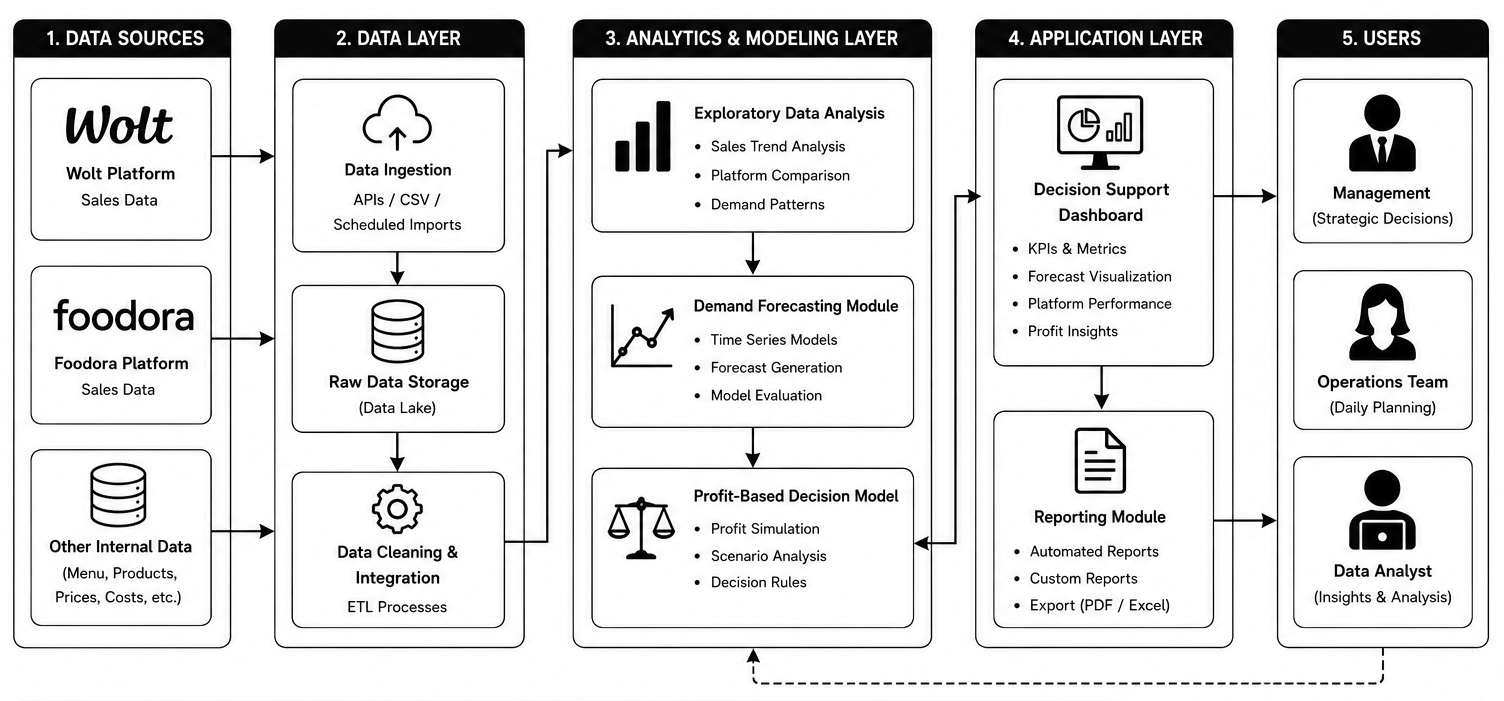
\includegraphics[width=\textwidth]{figures/System_Architecture.png}
\caption{System Architecture of the Proposed Data-Driven Decision Support Framework for Third-Party Delivery Sales}
\label{fig:architecture}
\end{figure}

\subsection{Data Collection}

This research employs historical sales data sourced from two third-party delivery platforms, specifically Wolt and Foodora. This includes transactional level data to understand the ordering trend, sales and demand at a platform level. These datasets are the building blocks for data analysis, prediction, and decision-support model creation.

\textbf{Wolt Dataset}

The Wolt data is from the historic sales records of wolt site. It includes data such as order date and time, sales value, and other relevant transaction data. Using this data we analyze demand behavior over time and build forecasting models at the platform level.

\textbf{Foodora Dataset}

Foodora also has the history of sale transactions data of the same type. Foodora platform. It provides information on when orders were placed, how many were sold and what features are important. This data is used alongside Wolt data for comparison and analysis, and to develop a joint forecasting and decision-support framework.


\subsection{Data Preprocessing}

The collected data needs to be preprocessed before analysis and model development to ensure accuracy and consistency. This step aims to improve data quality and prepare it for forecasting and optimization, so data preprocessing is an essential step.

\textbf{Data Cleaning}

Data cleaning is the processes of detecting and correcting (or removing) corrupt or inaccurate records from the dataset. It is about missing values, removing duplicate records and correcting the almost accurate records. Cleaning ensures the data is reliable and does not hold a bias towards model performance.

\textbf{Data Integration}

Data integration is the union of datasets that are given through more than one sources into one coherent single dataset. Since in this work sales info about Wolt and Foodora is going to be merged together to a single dataset. This allows for a consistent analysis across platforms and enables the construction of an overall forecasting- and decision support model.

\textbf{Feature Engineering}

Feature engineering is creating new ones or modifying existing ones to improve model performance. Examples Include features based on time as day of the week or month and hence extract features lag variables or computes sales sums. These features allow forecasting models to be more predictive and better capture the nature of patterns.

\subsection{Mathematical Formulation}
The mathematical formulations in this study are used to support the demand forecasting and the decision-making for profit in the proposed framework. Mathematical modeling can be used to provide a structured representation of sales behavior, forecasting performance, and profitability of a business \citep{botchkarev2018performanc}. These formulations offer a quantitative basis to analyse historical sales data from third-party delivery platforms. In the forecasting aspect of the study, it is assumed that future sales demands can be predicted from past sales pattern. The general forecasting function is represented as:
\begin{equation}
\hat{Y}_t = f(X_t)
\end{equation}

where $\hat{Y}_t$ represents the predicted sales value at time $t$, and $X_t$ is the historical sales observations and related variables used as input for the forecasting model. The purpose of the forecasting process is to recognize trends and recurring demand patterns from past transactions. To be able to forecast future sales. Sales demand can be further represented with trend, seasonal and irregular components (time-series behavior).:
\begin{equation}
Y_t = T_t + S_t + E_t
\end{equation}

where $Y_t$ represents the observed sales value at time $t$, $T_t$ is the long-term trend component, $S_t$ denotes seasonal variations, and $E_t$ indicates the random error component. This formulation supports the analysis of periodic demand fluctuations commonly observed in restaurant sales and food delivery platforms \citep{chai2014rooc}. In addition to forecasting, the framework includes a profit-oriented
decision model. The general profit equation is expressed as:
\begin{equation}
P = R - C
\end{equation}
where $P$ represents total profit, $R$ is called revenue generated from sales, and $C$ is the operational costs.
The objective of this formulation is to evaluate how forecasted sales demand may influence business profitability and managerial decision-making. The profit formulation can be extended to include item-level sales
performance:

\begin{equation}
P = \sum_{i=1}^{n}(S_i \times M_i) - C
\end{equation}

where $S_i$ denotes the sales volume of item $i$,
$M_i$ denotes the profit margin associated with item $i$,
and $C$ refers to total operational costs. This formulation enables the evaluation of product-level profitability and supports data-driven sales optimization.
To assess forecasting accuracy, evaluation metrics are incorporated into the framework. One commonly used metric is Mean Absolute Error (MAE), which measures the average prediction error:
\begin{equation}
MAE = \frac{1}{n}\sum_{i=1}^{n}\left|Y_i - \hat{Y}_i\right|
\end{equation}

where $Y_i$ represents the actual sales value and $\hat{Y}_i$ represents the predicted sales value. Lower MAE values indicate higher forecasting accuracy. Another important metric is Root Mean Square Error (RMSE), defined as:
\begin{equation}
RMSE = \sqrt{\frac{1}{n}\sum_{i=1}^{n}(Y_i - \hat{Y}_i)^2}
\end{equation}

RMSE measures the square root of the average squared forecasting error and gives greater importance to larger prediction deviations \citep{hodson2022root}. These evaluation metrics provide a systematic approach for comparing forecasting performance and validating the effectiveness of the proposed
analytical framework.

\subsection{Analytical Framework}

The research is based on a systematic analysis procedure which converts raw sales information into actionable decision support. The framework comprises of four key steps: data integration, descriptive analysis, predicting, and optimization.

The first step involves data integration whereby sales data of Wolt and Foodora are integrated into a.
single unified dataset. This makes it consistent and it can be analyzed on a number of platforms. Second, descriptive analysis is done to comprehend past sales trends. This involves finding trends, seasonal factors and platform differences. The objective of this step is to learn about the previous performance and to prepare the data to.
forecasting.

Third, there are forecasting models which are formulated to forecast future demand at the platform level. Various time series and machine learning methods are used and tested to identify maximize the best model. The basis of decision-making is based on these forecasts.
Lastly, optimization will be used to produce profit-oriented recommendations. Using the predicted demand, a decision model is created to aid in activities like platform level allocation or promotion planning.

This is where predictions are converted into actionable decisions which are meant to add value to business performance. In general, this analytical framework ties data, models and decisions into one process, allowing a shift in data analysis to data-driven decision-making..


\begin{figure}[h]
\centering
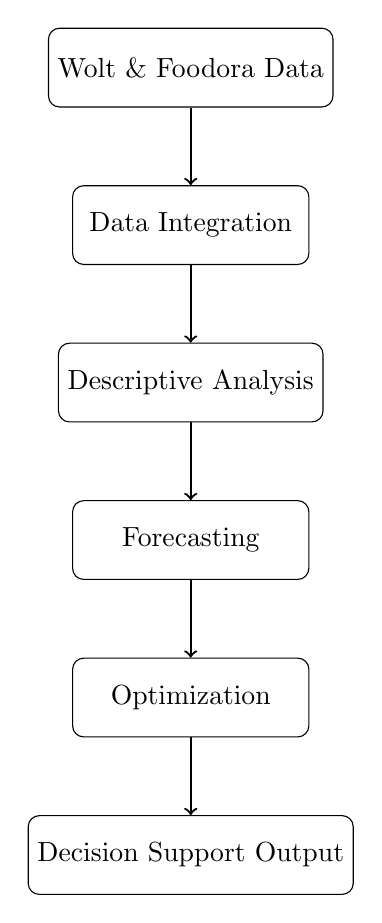
\begin{tikzpicture}[
    node distance=2cm,
    every node/.style={draw, rectangle, rounded corners, align=center, minimum width=3cm, minimum height=1cm},
    arrow/.style={->, thick}
]

\node (data) {Wolt \& Foodora Data};
\node (integration) [below of=data] {Data Integration};
\node (descriptive) [below of=integration] {Descriptive Analysis};
\node (forecasting) [below of=descriptive] {Forecasting};
\node (optimization) [below of=forecasting] {Optimization};
\node (decision) [below of=optimization] {Decision Support Output};

\draw[arrow] (data) -- (integration);
\draw[arrow] (integration) -- (descriptive);
\draw[arrow] (descriptive) -- (forecasting);
\draw[arrow] (forecasting) -- (optimization);
\draw[arrow] (optimization) -- (decision);

\end{tikzpicture}
\caption{Analytical Framework of the Study}
\end{figure}
\newpage
\section{Descriptive Data Analysis}

\subsection{Dataset Overview}

A dataset, comprising a combination of historical sales data of Wolt and Foodora, is used in this study. The sample size was mostly restricted to one vendor because it was not possible to reach various branches. The study can be further extended with more data. Foodora, on the other hand, is any other competitive party of the existing delivery services.

The final dataset, having been cleaned and integrated, is a structured, transaction record, which is analyzed and developed into a model. The database comprises of a total number of records of individual orders during the period of time chosen. A record is associated with every transaction and it contains details regarding sales and time.

The dataset contains several key variables. They usually include order date and time, sales value, platform identifier (Wolt or Foodora), and other features that are developed in the course of preprocessing, including day of the week or month. Patterns are analyzed with these variables and help to predict models.

The data includes a certain period of time, and the study enables the researcher to record the trends and seasonal changes in the demand. This window is critical in determining the customer behavior changes and making sure that the forecasting models are trained of adequate historical information. 

All in all, the data set gives a full picture of the platform-level sales activity and is the foundation of descriptive analysis, forecasting and optimization in this research.


\subsection{Sales Patterns}

This section analyzes the historical sales data to identify important patterns in customer demand. Understanding these patterns helps in building accurate forecasting models and supports better decision-making.

\begin{table}[h]
\centering
\begin{tabular}{|p{4cm}|p{10cm}|}
\hline
\textbf{Category} & \textbf{Description} \\
\hline
Daily Order Trends & Shows how the number of orders changes day by day. It helps identify fluctuations in demand, including peaks and low periods influenced by factors such as promotions, holidays, or external events. \\
\hline
Weekly Patterns & Examines how demand varies across different days of the week. Typically, higher demand is observed on weekends, while weekdays show more stable but lower demand. This helps capture weekly seasonality. \\
\hline
Platform Comparison & Compares sales performance between Wolt and Foodora. It highlights differences in order volume, trends, and platform-specific demand, supporting better platform-level decision-making. \\
\hline
\end{tabular}
\caption{Summary of Sales Patterns}
\end{table}


\subsection{Exploratory Data Analysis (EDA)}

Exploratory Data Analysis (EDA) is done to understand the characteristics of the dataset, and to find out the key relationship between the data. It helps to visualize behavior of orders with time and helps to choose appropriate forecasting models.


In this study, various graphical analyses are employed. First is How are Order Values Distributed over Different Transactions while Being Associated with Orders. This help in checking if the data is skewed or either outliers.


Second, the order volatility of the networks is explored to investigate to what extent demand changes with time. Very high volatility means volatile demand while low volatility means the ordering patterns are more stable. Volatility is an important concept, to measure the difficulty of predicting.


Third, trend patterns are explored using time series plots. These plots show the volume of orders as a function of time and help to identify long-term trends, seasonal effects, and sudden shifts in demand. The historical order trend from the dataset we analyzed is shown in Fig.~\ref{fig:historical_orders}. The graph displays demand over time, showing demand patterns, peaks, drops, and seasonality among others.

Overall, the EDA provides valuable insights into the structure and behavior of the data, forming the foundation for the forecasting and optimization steps in this study.


\begin{figure}[h]
\centering
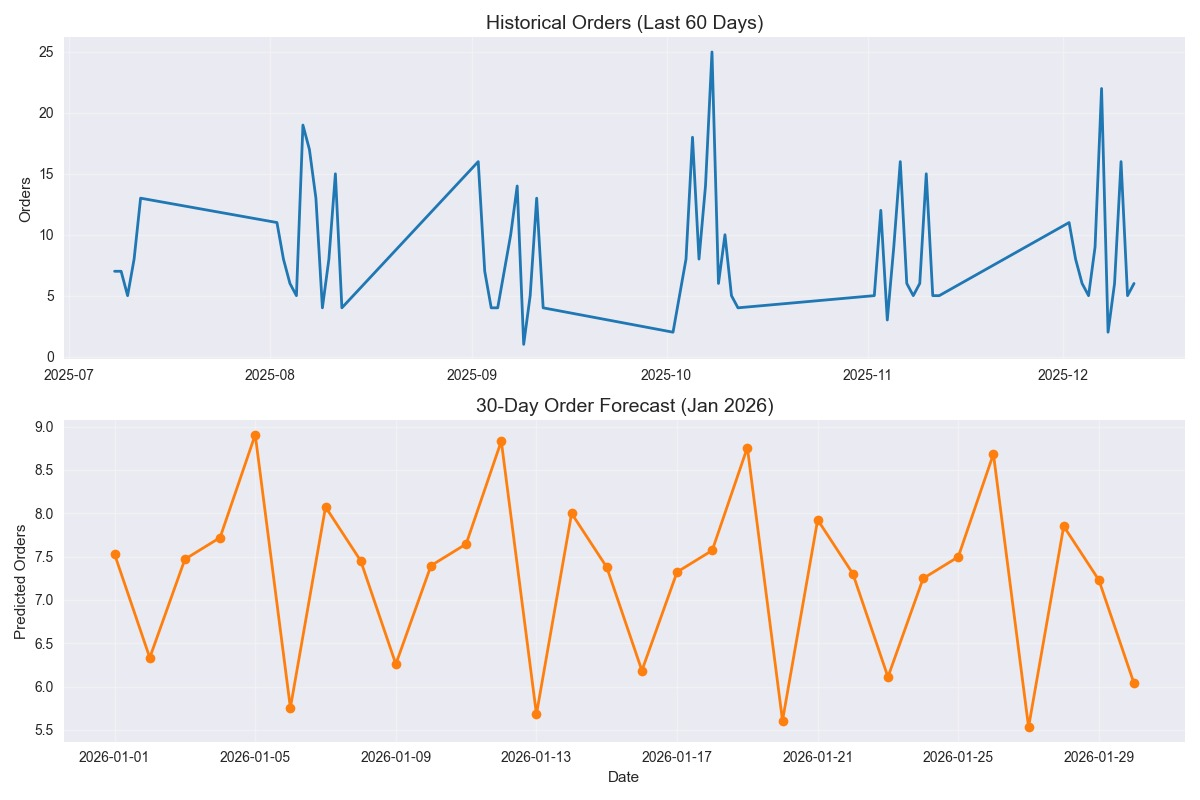
\includegraphics[width=0.9\textwidth]{figures/1.jpeg}
\caption{Historical Order Trends}
\label{fig:historical_orders}
\end{figure}
\newpage
\section{Demand Forecasting Model}

\subsection{Forecasting Approach}

In this work, the Prophet forecasting model is utilized to forecast the future demand in the sales of the third-party delivery platform. Prophet is chosen as it is suitable with business time series data and can process typical patterns like trends and seasonality. 

The possibility to model the time series data having a high seasonal influence, e.g. daily and weekly trends is one of the primary reasons why Prophet is selected. This feature can be especially helpful in the case of food delivery platforms, where demand tends to change on a weekly basis. Prophet is able to automatically record these patterns without the need to make any manual adjustments. 

The other strength of Prophet is that it can withstand missing data and outliers. Sales data in real-life scenarios tend to have anomalies and Prophet is set to manage these anomalies. This renders it viable to use in business applications in which data might not be exactly clean. 

Also, Prophet can be implemented and interpreted easily as opposed to other more complicated machine learning models. It has well-defined elements like trend and seasonality that can be used to explain how the model has come up with forecasts. The transparency is necessary in terms of decision-making and reporting the outcomes to the stakeholders. 

Lastly, Prophet works reasonably well with rather small data and involves little parameter optimization. This renders it appropriate in this study, in which the objective is to come up with a robust and useful forecasting model to be used in decision-support. In general, Prophet is selected as it is accurate, simple, and interpretable and is a suitable tool in forecasting the platform-level demand in this study.


\subsection{Model Specification}

The Prophet model decomposes the time series into several key components, mainly trend, seasonality, and holiday effects. These components help capture different patterns in the data and improve forecasting accuracy.

\textbf{Trend Component}

The trend component is the long term trend of the time series. It shows
whether the level of orders is tending upwards, downwards, or is in a steady state over time. Prophet fits a piecewise linear or logistic growth function to model the trend to enable it to record both incremental and abrupt changes in the data. This is important of business data in which demand can vary based on market conditions or business.
strategies.

\textbf{Seasonality}

Seasonality reflects recurring patterns, which are periodically repeated. Weekly seasonality is especially significant in this research because the behavior of customers in terms of ordering can be very different on different days of the week. As an illustration, the demand can be greater during the weekends than weekdays. Prophet uses flexible functions to automatically model these seasonal patterns thus enabling it to capture and model changes in demand which are periodic.

\textbf{Holiday Effects}

Holiday effects explain unusual events that might have an impact on the demand like a special occasion or a public holiday. The behavior of customers during such times can be far off the normal trend and as a result, orders may peak or decline. Prophet enables consideration of the variables of holidays to modify the forecasts. Holiday effects may be used in this study provided that there is the relevant data, but its effect may be minimal depending on the data.


\subsection{Forecast Results}

This section presents the results obtained from the Prophet forecasting model. The results are analyzed through trend, seasonality, and forecasted demand to understand future sales behavior.

\textbf{Trend Analysis}

The trend component shows the overall direction of demand over time. Based on the Prophet model, the trend indicates a slight downward pattern in the number of orders over the observed period. This suggests that, on average, demand is gradually decreasing, although short-term fluctuations still occur.

Figure~\ref{fig:trend_component} illustrates the estimated trend component from the model.

\begin{figure}[h]
\centering
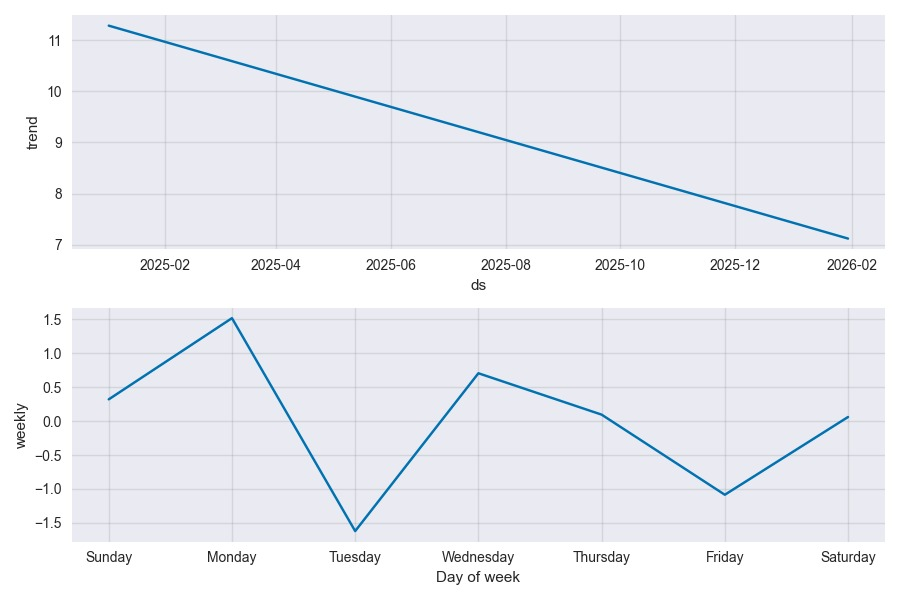
\includegraphics[width=0.8\textwidth]{figures/2.jpeg}
\caption{Trend Component from Prophet Model}
\label{fig:trend_component}
\end{figure}


\textbf{Weekly Seasonality}

The weekly seasonality component captures how demand changes across different days of the week. The results show that demand is higher on certain days (such as weekends or early weekdays) and lower on others. For example, Monday and Wednesday may show higher demand, while Tuesday and Friday show lower demand.

This pattern reflects customer behavior and is important for understanding recurring demand cycles.

Figure~\ref{fig:weekly_seasonality} presents the weekly seasonal pattern.

\begin{figure}[h]
\centering
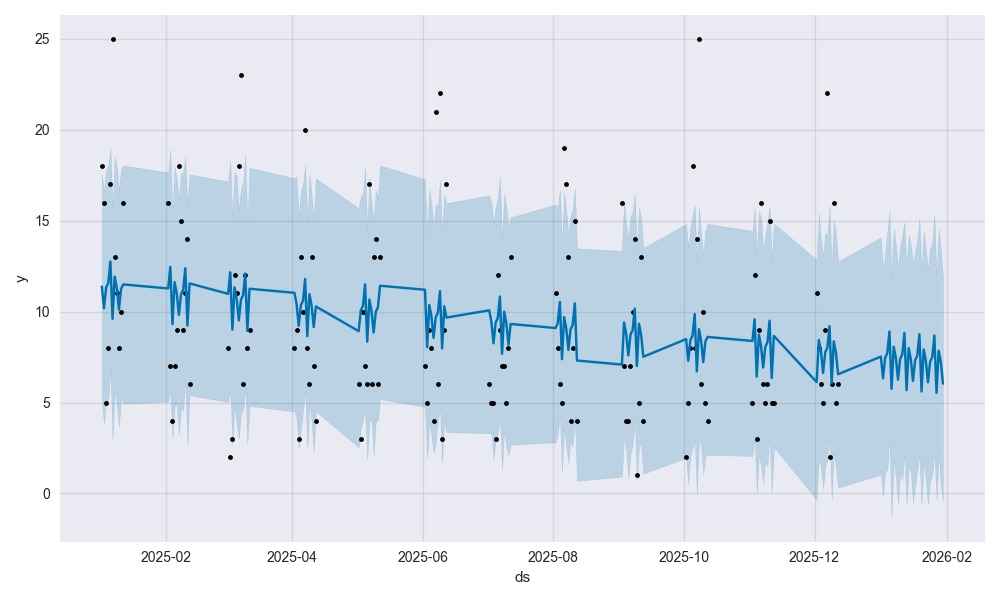
\includegraphics[width=0.9\textwidth]{figures/3.jpeg}
\caption{Weekly Seasonality from Prophet Model}
\label{fig:weekly_seasonality}
\end{figure}


\textbf{Forecasted Demand}

The forecasted demand shows the predicted number of orders for the future period. The model predicts relatively stable demand with moderate fluctuations, typically ranging within a consistent interval. Compared to historical data, the forecast appears smoother, indicating that the model reduces random noise while capturing underlying patterns.

Figure~\ref{fig:forecast} shows the full forecast, including historical data, predicted values, and confidence intervals.

\begin{figure}[h]
\centering
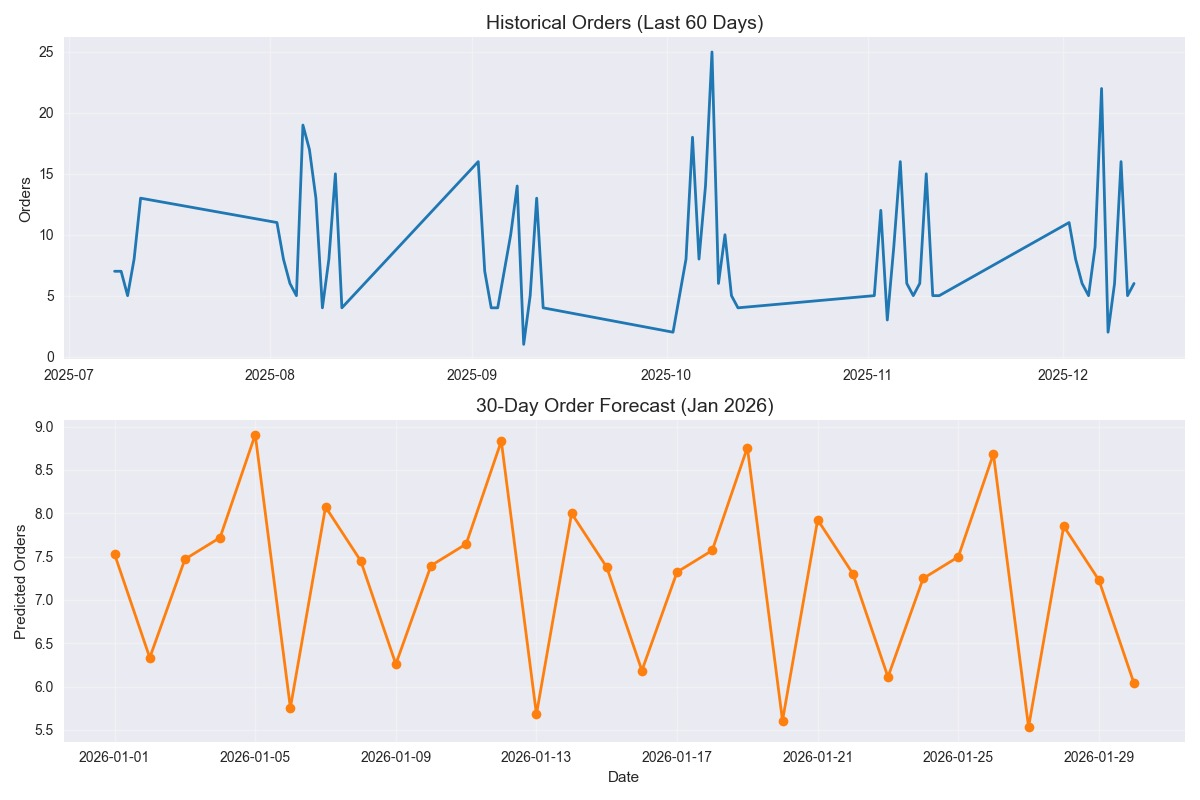
\includegraphics[width=1.0\textwidth]{figures/4.jpeg}
\caption{Forecasted Demand using Prophet}
\label{fig:forecast}
\end{figure}

Overall, the results demonstrate that the Prophet model effectively captures trend and seasonal patterns while providing reliable forecasts for future demand.


\subsection{Forecast Accuracy Evaluation}

To evaluate the performance of the forecasting model, several standard accuracy metrics are used. These metrics compare the predicted values with the actual observed values and help assess how well the model performs.

\begin{table}[h]
\centering
\begin{tabular}{|p{4cm}|p{4cm}|p{6cm}|}
\hline
\textbf{Metric} & \textbf{Definition} & \textbf{Description} \\
\hline
MAE (Mean Absolute Error) & Average of absolute differences between actual and predicted values & Measures overall prediction error in simple terms. Easy to interpret. Lower values indicate better accuracy. \\
\hline
RMSE (Root Mean Squared Error) & Square root of average squared differences between actual and predicted values & Penalizes larger errors more than MAE. Sensitive to outliers. Lower values indicate better performance. \\
\hline
MAPE (Mean Absolute Percentage Error) & Average percentage difference between actual and predicted values & Expresses error as a percentage, making it easy to understand and compare. Can be sensitive when actual values are very small. \\
\hline
\end{tabular}
\caption{Forecast Accuracy Metrics}
\end{table}
\newpage
\section{Prescriptive Decision Model}

\subsection{Decision Problem Definition}

The primary decision issue within this paper is the allocation of the sales or promotion activities across various delivery platforms to the maximum profit. As platforms like Wolt and Foodora have a dissimilar commission framework, demand patterns, and customer behavior, it becomes significant to select the most suitable allocation strategy. 

In the absence of a systematic strategy, decisions can be based on intuition that can result in inefficiency in the utilization of resources and diminished profitability. Thus, a decision model grounded in data is required to aid in platform-level planning and enhance business performance.


\subsection{Optimization Model}

The optimization model is developed to transform demand forecasts into actionable decisions. It uses forecasted demand as input and generates recommendations that aim to maximize profit under given constraints.

\textbf{Objective Function}

The objective of the model is to maximize total profit. This is achieved by selecting the best allocation of orders or promotional efforts across platforms while considering revenues and costs. The objective of the model is defined as:

\[
\max \sum_{i} (Revenue_i - Cost_i) \cdot x_i
\]

where \(x_i\) represents the number of orders allocated to platform \(i\).


\textbf{Constraints}

The optimization model is subject to the following constraints:

\[
\sum_i x_i \leq Capacity
\]

\[
x_i \leq Demand_i
\]

The constraints can be explained as follows:

\begin{itemize}
    \item \textbf{Delivery capacity:} The total number of orders that can be handled is limited by operational capacity.
    
    \item \textbf{Platform fees:} Each platform charges different commission rates, which affect profit margins.
    
    \item \textbf{Demand limits:} The number of orders allocated to each platform cannot exceed the forecasted demand.
\end{itemize}

These constraints ensure that the model produces realistic and feasible recommendations.


\subsection{Decision Intelligence Framework}

The suggested model unites data, forecasting, and optimization into one pipeline. This is initiated by the launch of data collection and integration across various platforms. This information is subsequently utilized to come up with demand projections by the Prophet model. 

The required demand is sent to the optimization model that determines the optimal allocation strategy that will maximize profit. Lastly, the system generates decision recommendations which can aid managerial actions. 

Overall, the framework can be described as having a systematic flow: Data → Forecast → Optimization → Decision recommendation. By doing so, businesses can stop analyzing data and start taking action and making decisions that are more effective and based on data.


\subsection{Simulation / Back-Testing}

Simulation or back-testing is done to assess the effectiveness of the proposed decision-support framework using historical data. Back-testing entails the use of the forecasting and optimization models to previous data and the result compared with the real results. 

In this analysis, the historical sales data will be separated into training and testing periods. The forecasting model is trained with historical data and then is applied to make forecasts of the demand within a chosen time. The forecasts are then fed into the optimization model to produce decision recommendations. 

The framework is assessed by comparing the simulated decisions and actual historical outcomes. The main indicators are evaluated, which are the accuracy of the forecasts and possible profit increase. This will enable the study to determine whether a better outcome would have been achieved in the event that the proposed model would have been implemented in real time. 

Simulation is useful to illustrate the practical usefulness of the framework without necessarily having to implement it in the actual world. It gives an illustration that the use of data-driven decisions can be more effective in enhancing performance than conventional or intuitive methods. 

On the whole, back-testing will guarantee that the proposed decision-support system is theoretically correct and practically effective to enhance the business decision-making process.
\newpage
\section{Results and Discussion}

\subsection{Forecasting Insights}

The demand analysis of the forecast shows that there are a few crucial trends in platform-level demand. Among the main findings is the existence of apparent differences in the weekly demand, as the number of demand differs by the day of the week. An example is that some days record higher order volumes and others have low demand. This is an indication of customer behavior and habitual consumption. 

Furthermore, the data has seasonal trends. The forecasting model captures the repeating patterns like weekly seasonality, meaning that demand has predictable patterns over time. The model can recognize the trends within the historical data and give consistent predictions, even though there are short-term changes and volatility. 

These observations prove that demand is not haphazard but capable of following specific patterns, and these can be used to plan and make decisions in a more efficient way.


\subsection{Optimization Results}

The recommendations for the optimization model are related to the allocation of orders and promotions among delivery platforms so as to maximize the profit. The findings show that each platform has a varying impact on overall business performance, as a result of variations in customer demand, platform commissions, and sales volume.

The optimization framework helps identify allocation strategies that focus on the more rewarding platforms while taking into account the expected demand constraints and operational limitations. The optimized allocation strategy is more effective in using business resources and marketing efforts than the equal allocation or the intuition-based allocation strategies.

The implementation of the optimization model based on the results of simulation and back testing, may lead to the potential for the improvement of profitability from historical decision making processes. The forecasting outputs are incorporated into the optimization process, which can help to minimize uncertainty caused by demand fluctuations and make more informed managerial decisions.

The results also show that forecast-based optimization can augment the promotional planning process by optimizing campaigns to the periods and platforms where more is expected to be gained from the promotion. This helps businesses to make the best use of their marketing budgets and boost their overall efficiency.

Yet another lesson to be learned is that the optimization model enables strategic platform assessment. The framework allows companies to assess the performance of the platforms apart from the number of sales to also measure the profitability contribution, thus further adding to the business performance. This analysis can help management determine which platforms are more valuable to the business and where investments and promotions should be made.

The optimization results indicate that business efficiency can be increased, strategic planning can be supported and operational performance can be optimized in a third-party delivery environment by combining forecasting with profit-oriented decision models.


\subsection{Business Implications}

The suggested decision support structure offers a number of implications for HungryHub Oy. The company can shift from reacting to making decisions towards a more proactive and data-driven approach to operations, by combining data analysis, forecasting, and optimization into a single analytical model.

This framework will enable the company to have a better understanding of the behaviour of customer demand; platform specific performance, and future sales. These insights help to make better plans for promotion, pricing and resource planning decisions for various delivery platforms.

Besides, the forecasting aspect helps management to forecast the change in demand and accordingly prepare operational resources. This could help in optimizing inventory planning, manpower utilization, and campaign scheduling, especially during peak seasons. Better visibility of forecasting could also help to mitigate operational uncertainty and avoid excess costs of over-preparing or underutilizing resources.

The optimization component helps improve profits through the evidence-informed allocation decisions. This framework allows for decisions to be made based on forecasted demand patterns and for a profitability analysis of the platform. This is not merely relying on managerial intuition. This helps to use marketing resources and operate more efficiently.

The framework is also useful in the long term business planning process. The company can constantly track the performance of the platform and sales trends, which can help them understand the preferences of their users and see how well their platform partnerships are working. This can help management to make adjustments to business strategies in the fast-expanding third-party delivery market.

The overall system showcases the potential of DDD to enhance operational efficiency, minimize uncertainty, and boost competitiveness in the digital food delivery landscape.

\subsection{Key Findings}
In this study, the main findings from the forecasting, optimization, and business analysis are summarized in Table \ref{tab:key_findings}. The results reveal key patterns of demand, platform level performance differences, and the opportunities for using forecasting and optimization techniques as part of business decisions. The summary also illustrates how the proposed framework can help enhance operational efficiency, improve profitability and support strategic planning in third party delivery settings.
\begin{table}[h]
\centering
\footnotesize
\renewcommand{\arraystretch}{1.6}
\setlength{\tabcolsep}{4pt}
\begin{tabular}{|p{4cm}|p{5.5cm}|p{4.5cm}|}
\hline
\textbf{Key Finding} & \textbf{Observation} & \textbf{Business Implication} \\ \hline

Weekly demand variation &
Customer demand differs across weekdays and weekends &
Supports better staffing and operational planning \\ \hline

Seasonal demand patterns &
Repeating sales trends were identified in historical data &
Enables improved forecasting and inventory preparation \\ \hline

Platform-level performance differences &
Wolt and Foodora showed different sales and profitability behaviors &
Assists in platform-specific strategic planning \\ \hline

Forecasting model effectiveness &
The forecasting model captured major demand trends with acceptable accuracy &
Supports data-driven demand prediction and planning \\ \hline

Optimization-based allocation &
Profit-oriented allocation produced better outcomes than historical allocation strategies &
Improves resource utilization and profitability \\ \hline

Forecast-driven decision-making &
Combining forecasting with optimization improved managerial insight &
Reduces uncertainty in operational decisions \\ \hline

Promotional planning opportunities &
High-demand periods can be identified in advance &
Enables more efficient promotional campaign scheduling \\ \hline

Data integration benefits &
Centralized analysis improved visibility across sales channels &
Supports comprehensive business monitoring \\ \hline

Strategic business value &
The framework supports proactive rather than reactive decision-making &
Enhances competitiveness in the delivery market \\ \hline

Scalability potential &
The framework can be extended into a real-time decision-support system &
Provides opportunities for future system development \\ \hline

\end{tabular}
\caption{Key Findings and Business Implications}
\label{tab:key_findings}
\end{table}

\subsection{Research Questions and Answers}

This section presents the main research questions of the study and explains how each question has been addressed based on the results.

\textbf{RQ1: How can sales data from third-party delivery platforms be structured into a unified analytical dataset?}

The study addressed this question by cleaning and integrating data from Wolt and Foodora into a single dataset. This unified dataset enabled consistent analysis across platforms and served as the foundation for forecasting and optimization.

\textbf{RQ2: Which forecasting approach provides the most accurate predictions of platform-level demand?}

The Prophet model was selected and applied due to its ability to capture trend and seasonal patterns effectively. The evaluation results showed that Prophet provides reliable and stable forecasts suitable for business decision-making.

\textbf{RQ3: How can demand forecasts be transformed into profit-oriented decision recommendations?}

The study developed an optimization model that uses forecasted demand as input. This model generates recommendations on how to allocate orders or promotional efforts across platforms to maximize profit under given constraints.

\textbf{RQ4: What is the potential business impact of a prescriptive decision-support framework in optimizing platform sales performance?}

The simulation and back-testing results indicate that the proposed framework can improve decision-making and increase potential profitability. By combining forecasting and optimization, the system provides more effective and data-driven recommendations compared to traditional approaches.
\newpage
\section{Conclusion}

This paper has created a prescriptive decision-support model to optimize the sales of third-party delivery platforms, based on the data provided by Wolt and Foodora. The findings revealed that decision making can be greatly enhanced through integration of data, the application of forecasting models and the application of optimization techniques. 

The forecasting model was able to determine the demand patterns of weekly seasonality and changes in the order volume. These forecasts were converted into actionable recommendations by the optimization model, and it showed the possibility of optimizing the profit by increasing the platform-level allocation. 

In general, the research establishes the fact that predictive and prescriptive analytics could be combined to offer a solid basis to data-oriented decision-making in the QSR industry. 

This research adds to the scholarly community in that it combines the forecasting and optimization into a Design Science Research model. It builds upon the existing research by integrating predictive analytics with prescriptive decision-making on the platform of third-party delivery. The gap in the multi-platform analysis in the data of food delivery is also discussed in the study. 

Practically, the research offers a systematic framework that can be applied by companies like HungryHub Oy to enhance decision-making process. The framework assists in converting raw sales information into actionable insights to aid in enhancing planning, allocation of resources, and optimization of profits across delivery platforms.


\section{Limitations and Future Work}

\subsection{Limitations}

The study has a number of limitations in spite of its contributions. First, the analysis is conducted with the help of a small set of data of two platforms only, Wolt and Foodora. Second, the model is based on platform-specific assumptions, including fixed commission structure and simplified constraints. Third, the framework is not subjected to real-time operational environment and is tested with historical data.


\subsection{Future Work}

There are several possible ways in which this research can be extended in the future. One direction you can take is in adding multiple restaurants or business units to improve generalization. The other alternative is to develop real time decision-supporting systems that can update their future forecasts and recommendations in real time.

Additionally, future research could include advanced optimization techniques, dealing with operational variables like staffing, inventory, and logistics for the implementation of the delivery.
\newpage
% lisää lukuja -- more chapters...





%%%%%%%%%%%%%%%%%%%%%%
% lähteet - references
% replace url with doi at bibliography

% settings

\newtoggle{bibdoi}
\newtoggle{biburl}
\makeatletter

\undef{\APACrefURL}
\undef{\endAPACrefURL}
\undef{\APACrefDOI}
\undef{\endAPACrefDOI}

\long\def\collect@url#1{\global\def\bib@url{#1}}
\long\def\collect@doi#1{\global\def\bib@doi{#1}}
\newenvironment{APACrefURL}{\global\toggletrue{biburl}\Collect@Body\collect@url}{\unskip\unskip}
\newenvironment{APACrefDOI}{\global\toggletrue{bibdoi}\Collect@Body\collect@doi}{}

\AtBeginEnvironment{thebibliography}{
 \pretocmd{\PrintBackRefs}{%
  \iftoggle{bibdoi}
    {\iftoggle{biburl}{\unskip\unskip \bib@doi}{}}
    {\iftoggle{biburl}{Retrieved from\bib@url}{}}
  \togglefalse{bibdoi}\togglefalse{biburl}%
  }{}{}
}
%\apptocmd{\sloppy}{\hbadness 10000\relax}{}{} %skip error message about too long urls

\newpage




\bibliography{example}


% to-do: space between urldate and url



% liitteet - appendices
\input{appendices.tex}

\end{document}